%% bare_adv.tex
%% V1.4
%% 2012/12/27
%% by Michael Shell
%% See: 
%% http://www.michaelshell.org/
%% for current contact information.
%%
%%*************************************************************************
%% Legal Notice:
%% This code is offered as-is without any warranty either expressed or
%% implied; without even the implied warranty of MERCHANTABILITY or
%% FITNESS FOR A PARTICULAR PURPOSE! 
%% User assumes all risk.
%% In no event shall IEEE or any contributor to this code be liable for
%% any damages or losses, including, but not limited to, incidental,
%% consequential, or any other damages, resulting from the use or misuse
%% of any information contained here.
%%
%% All comments are the opinions of their respective authors and are not
%% necessarily endorsed by the IEEE.
%%
%% This work is distributed under the LaTeX Project Public License (LPPL)
%% ( http://www.latex-project.org/ ) version 1.3, and may be freely used,
%% distributed and modified. A copy of the LPPL, version 1.3, is included
%% in the base LaTeX documentation of all distributions of LaTeX released
%% 2003/12/01 or later.
%% Retain all contribution notices and credits.
%% ** Modified files should be clearly indicated as such, including  **
%% ** renaming them and changing author support contact information. **
%%
%% File list of work: IEEEtran.cls, IEEEtran_HOWTO.pdf, bare_adv.tex,
%%                    bare_conf.tex, bare_jrnl.tex, bare_jrnl_compsoc.tex,
%%                    bare_jrnl_transmag.tex
%%*************************************************************************


\documentclass[12pt,journal,compsoc]{IEEEtran}

\usepackage[utf8]{inputenc}
\usepackage{listings}
\usepackage{hyperref}
\usepackage{graphicx}
\usepackage{float}
\usepackage{enumitem}
\usepackage[svgnames]{xcolor}
\usepackage{color}

\definecolor{pblue}{rgb}{0.13,0.13,1}
\definecolor{pgreen}{rgb}{0,0.5,0}
\definecolor{pred}{rgb}{0.9,0,0}
\definecolor{pgrey}{rgb}{0.46,0.45,0.48}
\hypersetup{
  colorlinks=false,
  linkbordercolor={white}
}

\lstset{language=Java,
  showspaces=false,
  showtabs=false,
  breaklines=true,
  showstringspaces=false,
  breakatwhitespace=true,
  commentstyle=\color{pgreen},
  keywordstyle=\color{pblue},
  stringstyle=\color{pred},
  basicstyle=\ttfamily,
}


\newcommand\MYhyperrefoptions{bookmarks=true,bookmarksnumbered=true,
pdfpagemode={UseOutlines},plainpages=false,pdfpagelabels=true,
colorlinks=true,linkcolor={black},citecolor={black},urlcolor={black},
pdftitle={Práctica 3},
pdfsubject={Programación Distribuida y Tiempo Real - Práctica 4},
pdfauthor={Lucas Di Cunzolo,Santiago Tettamanti},
pdfkeywords={Programación Distribuida y Tiempo Real, java, LaTeX, jade}}

\hyphenation{op-tical net-works semi-conduc-tor}

\begin{document}
\title{Práctica 4\\Programación Distribuida y Tiempo Real}
\author{Lucas Di Cunzolo\\Santiago Tettamanti}

\IEEEtitleabstractindextext{%
\begin{abstract}
JADE
\end{abstract}

\begin{IEEEkeywords}
Programación Distribuida y Tiempo Real, java, \LaTeX, JADE
\end{IEEEkeywords}}

\maketitle

\IEEEdisplaynontitleabstractindextext
\IEEEpeerreviewmaketitle

\section{Punto 1}

\textit{Programar un agente para que periódicamente recorra una secuencia
        de computadoras y reporte al lugar de origen}
\begin{enumerate}[label=\alph* -]
  \item El tiempo total del recorrido para recolectar la información
  \item La carga de procesamiento de cada una de ellas.
  \item La cantidad de memoria total disponible.
  \item Los nombres de las computadoras.
\end{enumerate}

Para este punto, se creó un agente que crea 10 containers, y agrega
sus ID a un \texttt{ArrayList}, agregando al final al container inicial.

Luego simplemente se itera sobre el \texttt{ArrayList}, juntando la información
del container en el que se encuentra. Para almacenar la información, se
creo una clase anidada (\texttt{ContainerInfo}). Al conseguir la información,
se guarda una instancia de esa clase en otro \texttt{ArrayList}.

Al terminar la iteración, nos encontraremos en el container origen, con
una lista de instancias de \texttt{ContainerInfo}.

Luego se recorre ese array, imprimiendo los valores encontrados.\\

\hyperref[section:code-punto1]{Ver apéndice de código, Sección Punto 1}

\hyperref[section:cap-punto1]{Ver apéndice de capturas, Sección Punto 1}

Para ejecutar, se debe levantar el \texttt{jade.Boot}, esto se puede hacer
mediante el comando \texttt{make}

Simplemente se puede ejecutar \texttt{make start-gui}
Luego, para ejecutar el punto, se puede ejcutar \texttt{make run-punto1}

\section{Punto 2}

\textit{Programe un agente para que calcule la suma de todos los números
almacenados en un archivo de una computadora que se le pasa como
parámetro. Comente cómose haríalo mismo con una aplicación
cliente/servidor. Comente quepasaría si hubiera otros sitios con
archivos que deben ser procesados de manera similar}

Para este punto, se programó un agente que recibe el nombre de una computadora,
y migra el agente.
Una vez en la computadora destino, se realiza la lectura del archivo,
junto con la suma.
Al finalizar, se retora al container origen, y se muestra el resultado.\\

\hyperref[section:code-punto2]{Ver apéndice de código, Sección Punto 2}

\hyperref[section:cap-punto2]{Ver apéndice de capturas, Sección Punto 2}

Para ejecutar, se debe levantar el \texttt{jade.Boot}, esto se puede hacer
mediante el comando \texttt{make}

Simplemente se puede ejecutar \texttt{make start-gui}
Luego, para ejecutar el punto, se puede ejcutar \texttt{make run-punto2}


\section{Punto 3}

\textit{Defina  e  implemente  con  agentes  un  sistema  de  archivos
distribuido  similar  al  de  las prácticas anteriores.}

Para este punto, se programó un agente que pueda recibir argumentos, y
en base a lo recibido, realiza diferentes acciones.

Al ser métodos java, se pudo reutilizar gran parte del la lógica de la
práctica anterior.

El agente comprende 4 acciones:
\begin{itemize}
  \item list: La acción más simple. Recibe un parámetro extra a la acción,
        que marca cual es el directorio a listar.
        Una vez parseados los argumentos, se realiza la migración al servidor
        (recordemos que nos encontramos en el cliente).
        Al terminar la migración, se leen los archivos del directorio, y se
        almcenan en una variable de instancia del agente. Luego se vuelve al
        cliente y se informa lo leído.
  \item read: Recibe 2 argumentos extra a la acción, que marcan el nombre del
        nuevo archivo y el nombre del archivo remoto (en ese orden)
        Una vez parseados los argumentos, se realiza la migración al serviodr.
        Al termionar la migración, se leen los primeros 2000 bytes del archivo,
        y el tamaño total del archivo a leer y se almacenan en variables de instancia.
        En el cliente, se realiza la copia de los 2000 bytes, y se consulta si el
        tamaño total del archivo es menor o igual al tamaño copiado (en la primer
        vuelta va a ser igual a 2000), de no ser asi, se suman a una variable de
        \texttt{bytes copiados}, y se realiza la migración al servidor.
        En el servidor se copian los siguientes 2000 bytes \texttt{a partir}
        de los bytes copiados.(Esta acción se repite tantas veces como 
        sea necesaria)\\
        \hyperref[section:code-punto3]{Ver apéndice de código, Sección Punto 3}

        \hyperref[fig:initial-file]{Ver apéndice de capturas, Sección Punto 3}
  
  \item write: Trabaja de igual manera que el read, pero a manera inversa,
        siendo el cliente del item anterior, el servidor, y el servidor del item
        anterior el cliente.
  \item readwrite: Trabaja de igual manera que ejecutar primer un read y lugo un
        write de ese archivo.
\end{itemize}

Para ejecutar, se debe levantar el \texttt{jade.Boot}, esto se puede hacer
mediante el comando \texttt{make}

Simplemente se puede ejecutar \texttt{make start-gui}

Luego, para interactuar con el servidor, se cuenta con el script \texttt{run}

Para ver la sección de ayuda del comando, se puede utilizar la flag \texttt{-h}

\newpage
\onecolumn
\appendix{Código Java}
\label{appendix:codigo-java}

\subsection{Punto 1}
\label{section:code-punto1}
\lstinputlisting[language=Java]{../punto1/AgentePunto1.java}

\subsection{Punto 2}
\label{section:code-punto2}
\lstinputlisting[language=Java]{../punto2/AgentePunto2.java}

\subsection{Punto 3}
\label{section:code-punto3}
\lstinputlisting[language=Java]{../punto3/AgentePunto3.java}

\newpage
\subsection{Capturas}
\subsubsection{Punto 1}
\label{section:cap-punto1}
\begin{figure}[H]
  \centering
  \label{fig:punto-1-migracion}
  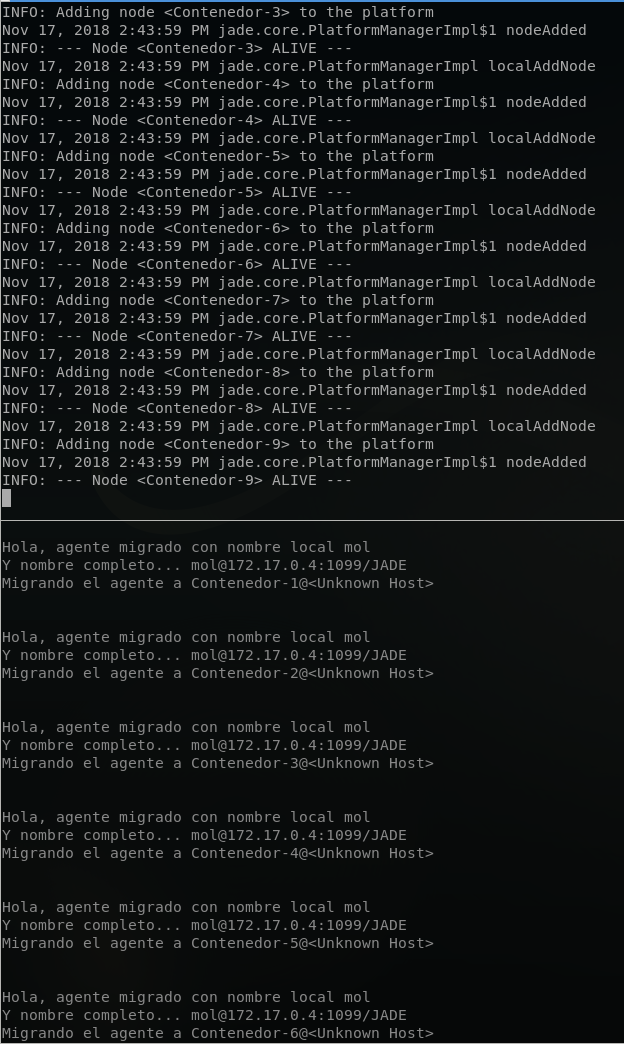
\includegraphics[width=90mm]{images/punto-1/1-migraciones.png}
  \caption{Migraciones}
\end{figure}

\begin{figure}[H]
  \centering
  \label{fig:punto-1-muestra}
  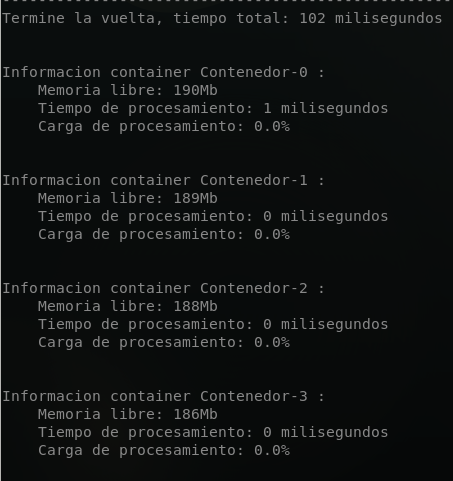
\includegraphics[width=90mm]{images/punto-1/2-muestra.png}
  \caption{Muestra de información}
\end{figure}

\subsubsection{Punto 2}
\label{section:cap-punto2}

\begin{figure}[H]
  \centering
  \label{fig:punto-2-archivo}
  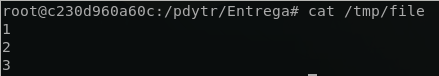
\includegraphics[width=90mm]{images/punto-2/1-archivo.png}
  \caption{Archivo a sumar}
\end{figure}

\begin{figure}[H]
  \centering
  \label{fig:punto-2-ejecucion}
  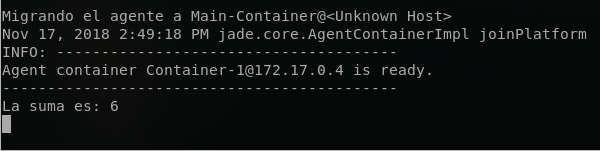
\includegraphics[width=90mm]{images/punto-2/2-ejecucion.png}
  \caption{Muestra de la suma}
\end{figure}


\subsubsection{Punto 3}
\label{section:cap-punto3}
\begin{figure}[H]
  \centering
  \label{fig:initial-file}
  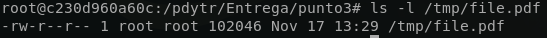
\includegraphics[width=90mm]{images/punto-3/1-initial-file.png}
  \caption{Inicio de copia}
\end{figure}

\begin{figure}[H]
  \centering
  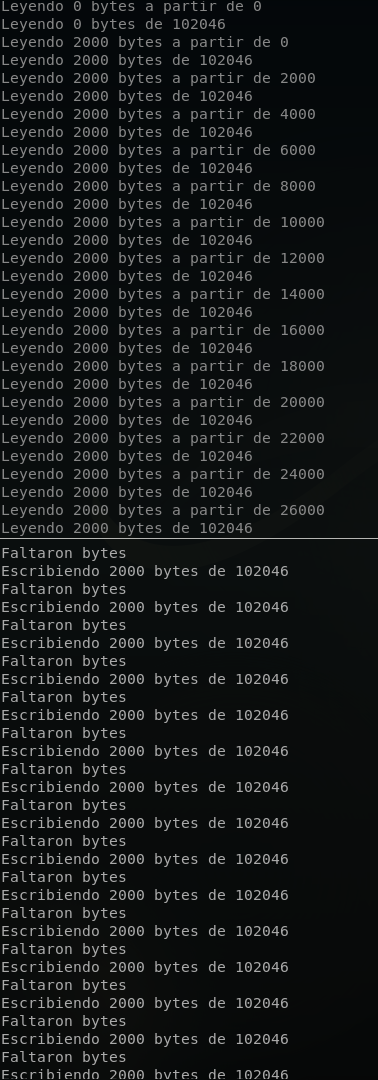
\includegraphics[width=75mm]{images/punto-3/2-start-read.png}
  \caption{Primera parte de la copia}
  \label{fig:start-read}
\end{figure}

\begin{figure}[H]
  \centering
  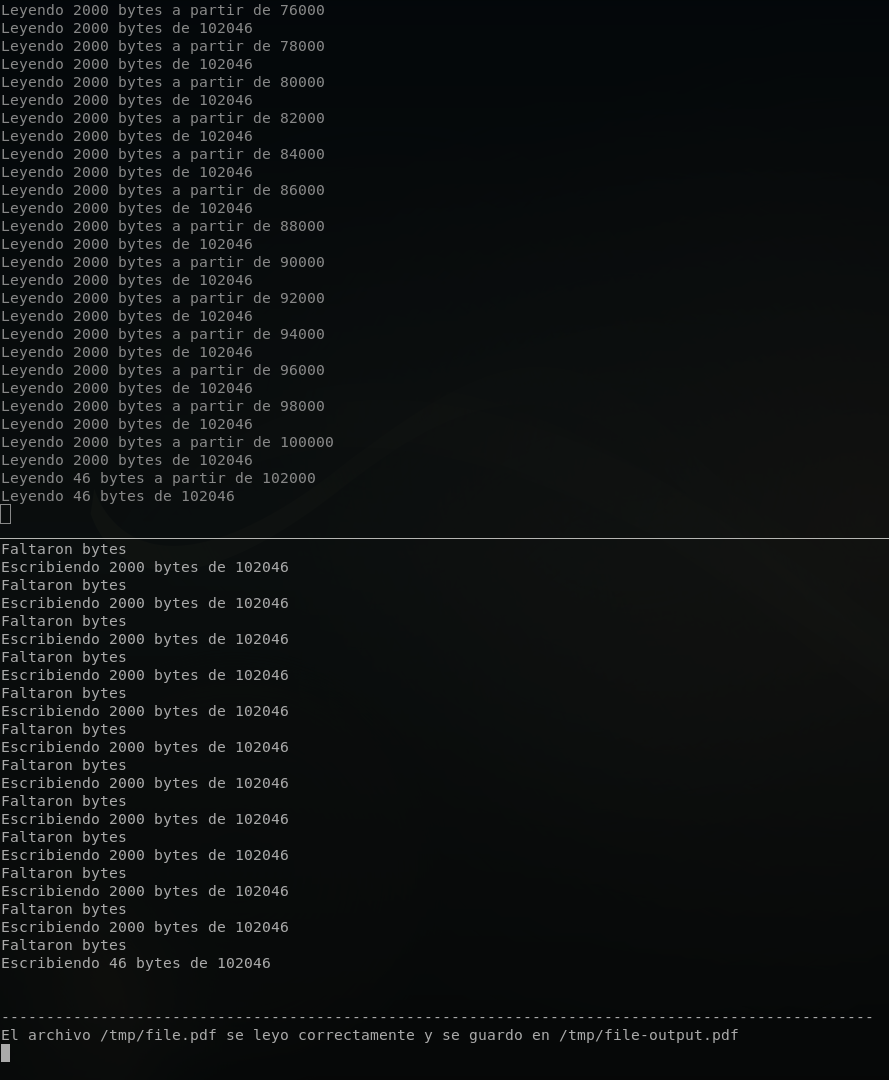
\includegraphics[width=160mm]{images/punto-3/3-end-read.png}
  \caption{Fin de la copia}
  \label{fig:end-read}
\end{figure}

\ifCLASSOPTIONcaptionsoff
  \newpage
\fi
\end{document}
